\documentclass[11pt,a4paper]{report}
\usepackage[latin1]{inputenc}
\usepackage{amsmath}
\usepackage{lipsum}
\usepackage{color}
\usepackage{listings, textcomp}
\usepackage{amsfonts}
\usepackage{amssymb}
\usepackage{graphicx}
\usepackage{longtable}
\usepackage{multirow}% http://ctan.org/pkg/multirow
\usepackage{hyperref}
\usepackage{gensymb}
\usepackage{pdflscape}
\hypersetup{colorlinks=true,allcolors=black}
\usepackage{tikz}
\usepackage{tikz-qtree}
\usepackage{hypcap}
\usepackage{cleveref}
\usepackage{amsmath}
\usepackage[export]{adjustbox}
\usepackage{tikz}
\usepackage{tikz-qtree}\usetikzlibrary{shapes.geometric, arrows}

\usepackage{placeins}
\usepackage{array}
\usepackage{subcaption}
\usepackage{footnote}
\usepackage{color,soul}
\newcolumntype{L}[1]{>{\raggedright\let\newline\\\arraybackslash\hspace{0pt}}m{#1}}
\newcommand{\note}[1]{\marginpar{\tiny{ \hl{#1 } } }  }

\usepackage{titlesec}
\titleformat{\chapter}[display]   
{\normalfont\huge\bfseries}{\chaptertitlename\ \thechapter}{20pt}{\Huge}   
\titlespacing*{\chapter}{0pt}{-50pt}{5pt}

\begin{document}

\begin{titlepage}
	\begin{center}
		\vspace*{-.5cm}
		\textsc{\LARGE Swinburne University of Technology}\\
		
		\begin{figure}[h]
			\centering
			
\includegraphics[width=0.5\linewidth]{swinburne_university_of_technology_111401}
		\end{figure}
		\vspace*{2cm}
		\hrule \  \\[0.4cm]
		\textsc{\Huge Hand-Eye Coordination Report}\\[0.5cm]
		\hrule \  \\[0.4cm]
		\textsc{\Large{RME 40003}\\ \  \\[0.1cm]
			\huge Robot System Design}\\[1cm]
		
		\normalsize
		\begin{tabular}{l r}
			\hline\\ Justin Sargent & 9989900 \\[0.25cm]
			\\ Phillip Smith & 7191731 \\ [0.25cm]
			\\ Thomas Rappos & 6336361 \\[0.25cm]
			\hline 
		\end{tabular} 
	\end{center}
\end{titlepage}
\tableofcontents
\chapter{Project Outline}
This project explores the use of a robotic arm used for pick-and-place automation tasks. For dynamic operation and task-completion feed-back, computer vision is incorporated via a web-cam mounted in the work area.\\
More specifically, this project has been completed for an industry client, AME System Pty. Ltd., for automated cavity pin insertion. These pins are 3.5mm wide and are placed in holes between 5 and 9mm apart on a rubber socket, as shown in \cref{fig:IMG_20160908_142218}(a) Due to this small size, a high degree of accuracy and repeatability is required.\\
\begin{figure}[h]
\centering
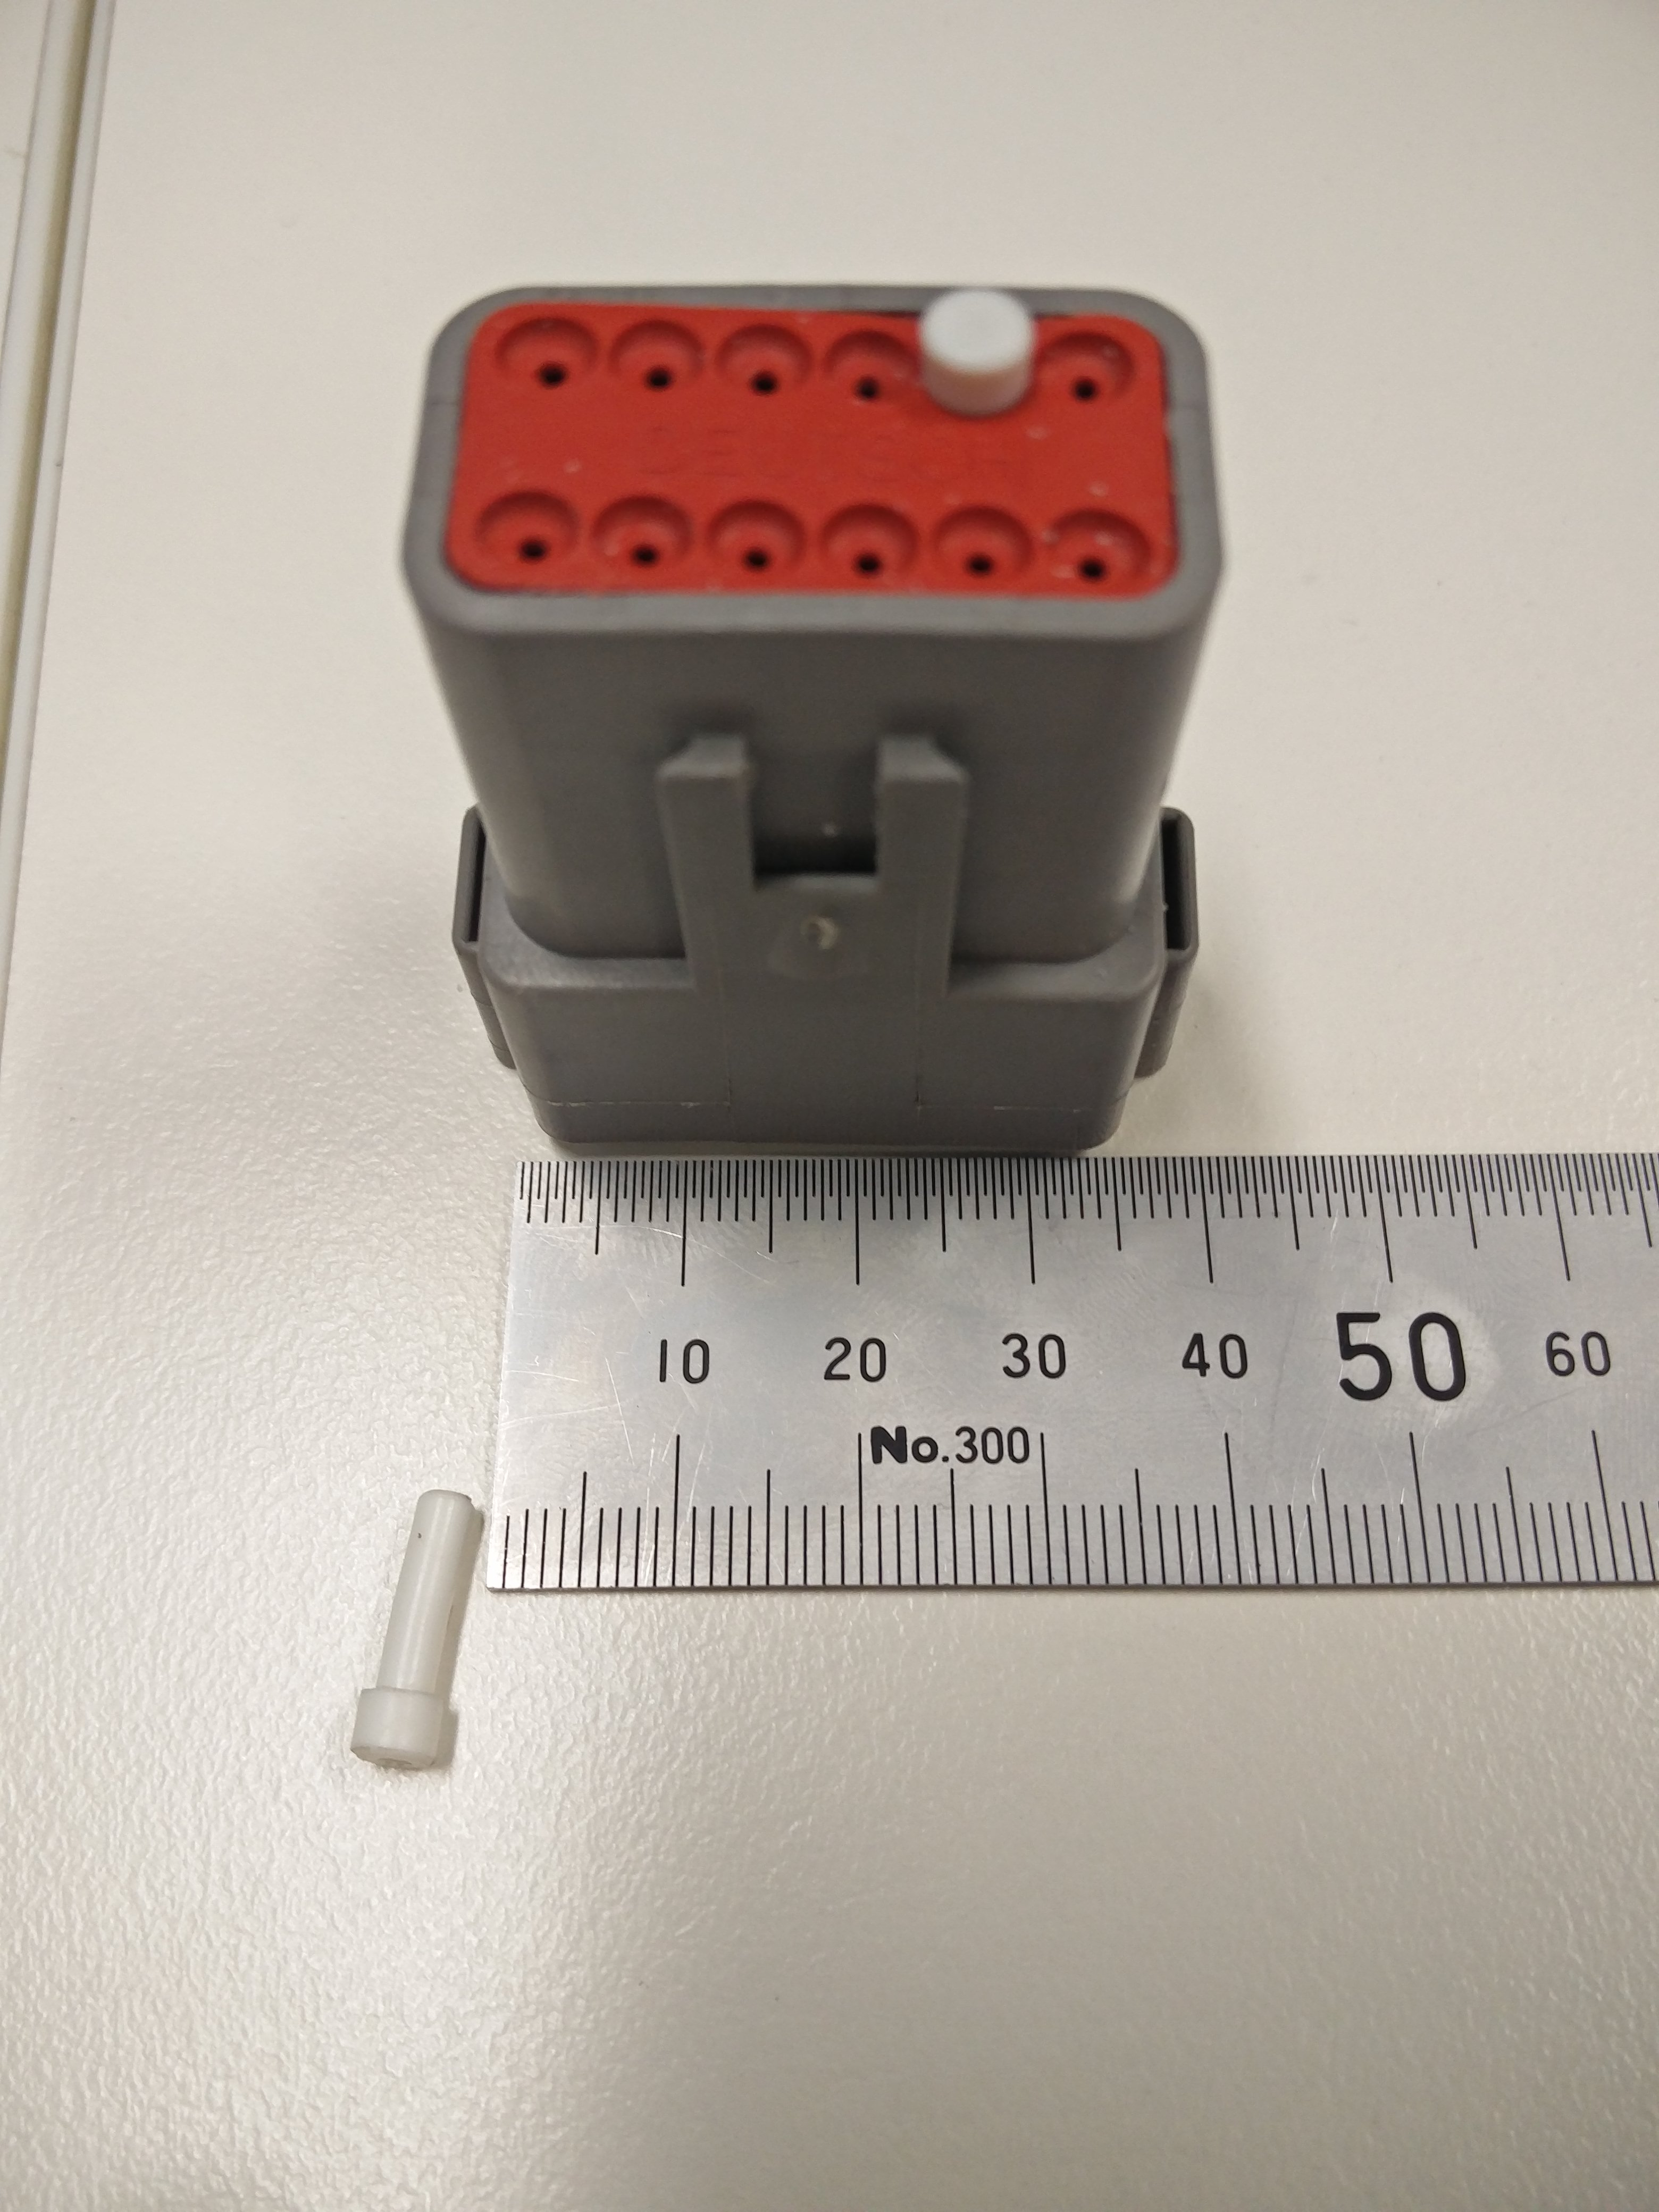
\includegraphics[width=0.25\linewidth]{IMG_20160908_142218} %
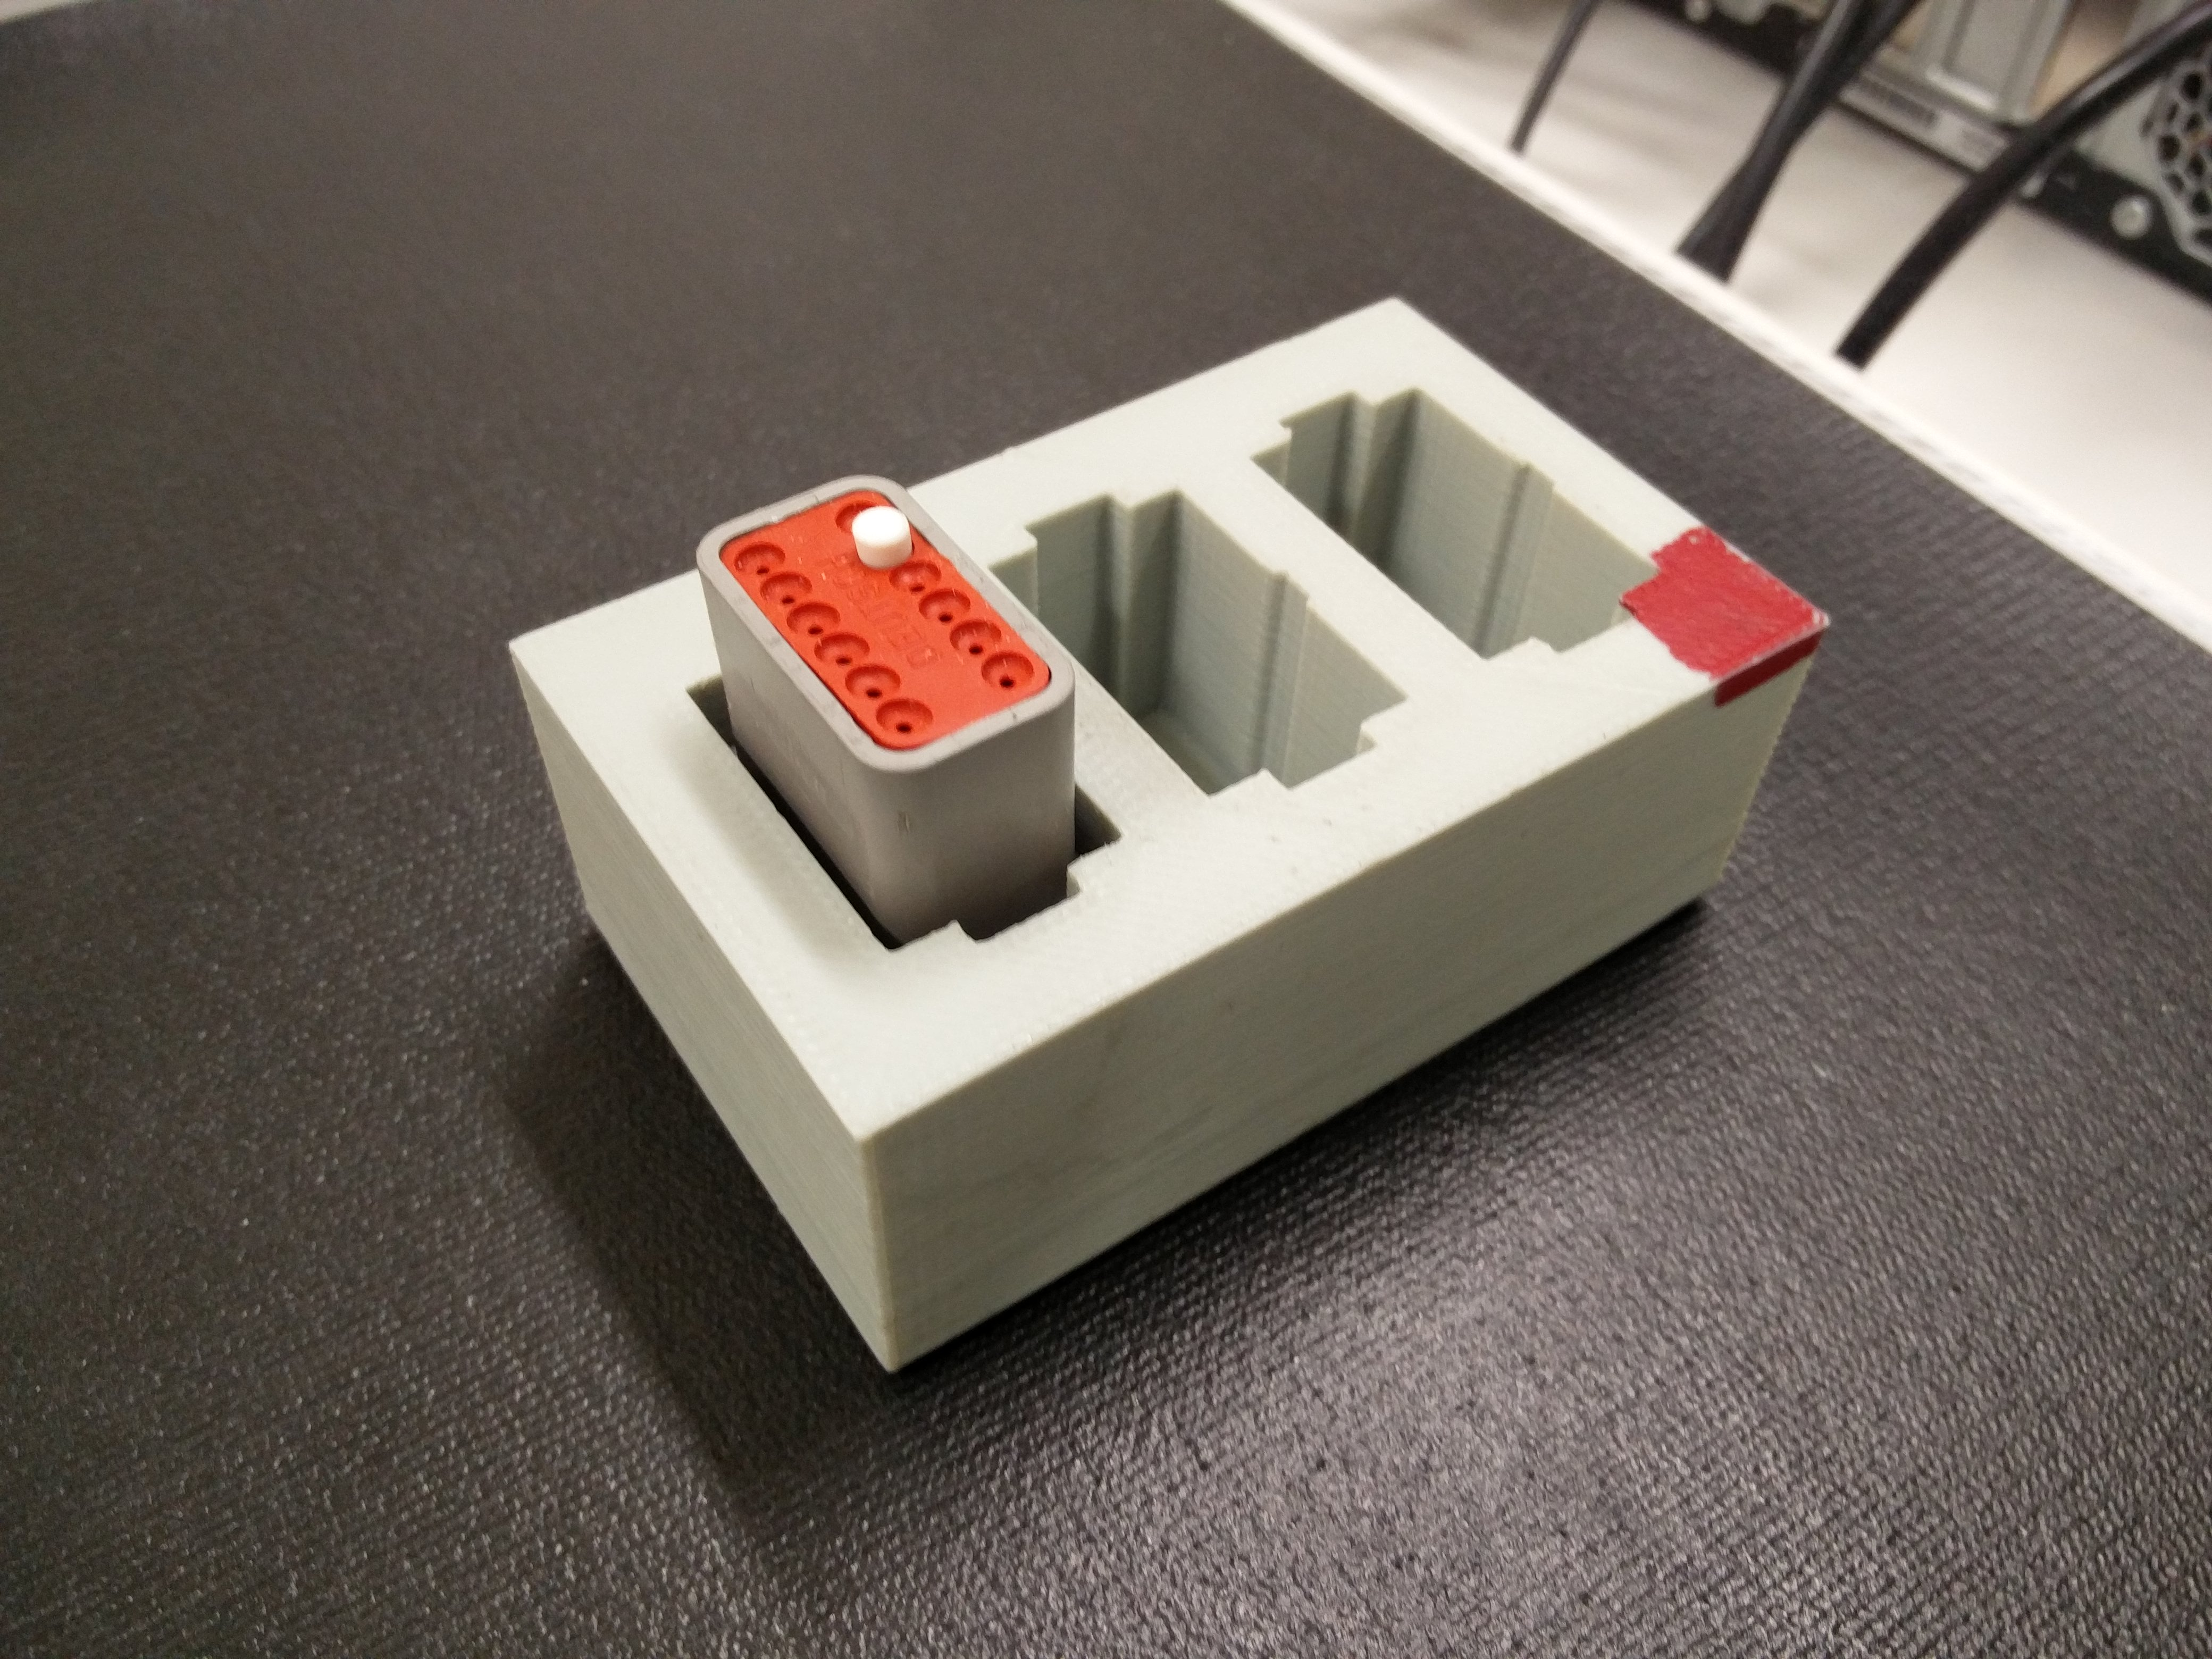
\includegraphics[width=0.45\linewidth]{IMG_20160912_135721}
\caption{Image of pin and socket, and socket in holding box}
\label{fig:IMG_20160908_142218}
\end{figure}
To hold the socket in place, and determine the orientation, a holding box has been produced which slots the sockets into a fixed position, shown in \cref{fig:IMG_20160908_142218}(b). For this project, these boxes are not themselves placed in a fixed location within the work space. As such the first objective of this project is using the computer vision to determine the global position of the pin holes, via the fixed position of the socket in the box, and the global position and orientation of the box in the work space.\\
The secondary objective is having the robotic arm collect a pin, and place it in the pin hole by converting the pinhole location in the camera frame to the required position in the robotic arm frame. The process for placing the pin with the robotic arm will then be as follows:
\begin{itemize}
\item Lower pin halfway into hole
\item Release pin
\item Drive pin remaining distance into hole.
\end{itemize}

For this project, the confirmation of pins being ready in the supply is not being explored. This is due to the industry application being intended to use a vibrating bowl feed, and thus the assumption can be made pins will always be available. For this proof of concept, a rack of three pins is made, with the gripper positions being hard coded.\\    

%\chapter{Gripper Design}
%With such small objects being handled, a custom gripper device was developed. The main gripper mechanism uses a Festo parallel, nematic gripper. While the gripping appendages have been custom made for this operation. Shown in \cref{fig:gripper2} are the open and closed CAD renderings of the gripper. Dark-grey being the Festo gripper, light grey being the main gripper appendage and green being the 3D printed gripper tips, modelled to specify grasp the cavity plugs.\footnote{two cavity plug sizes were initially requested}

%
%\begin{figure}[h]
%\centering
%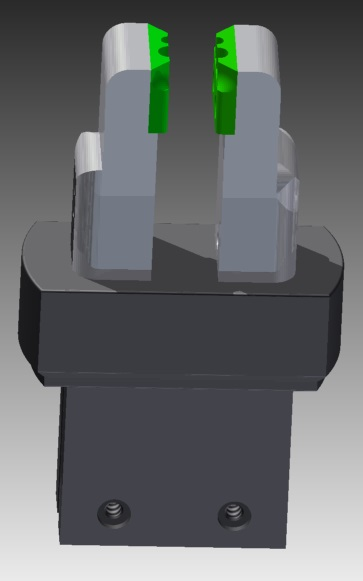
\includegraphics[width=0.4\linewidth]{gripper2}\ %
%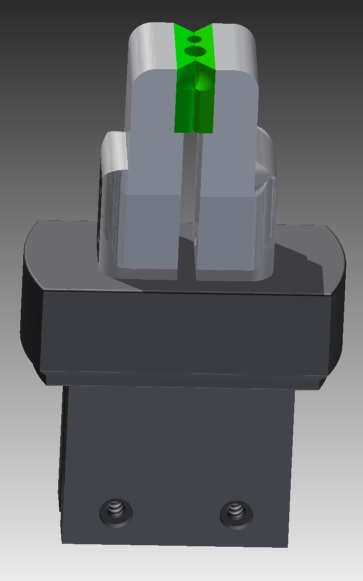
\includegraphics[width=0.4\linewidth]{gripper1}
%\caption{CAD rendering of plug gripper}
%\label{fig:gripper2}
%\end{figure}


\chapter{Computer Vision}
The computer vision of this project uses Open-CV for c++. This library contains many image-based functions for sourcing, manipulating, and presenting visual data. This library has been used for two roles, object detention, and robotic gripper required motion determination. Of these two task, the latter relies on the former. 
\section{Object detection}
\subsection{Environment preparation}
To begin the computer vision process a background image is taken when no objects are present. A keyboard control was added, 'Y', which allows a new background to be set. This was seen to be useful, as a background image taken on start-up, would often be too bright. This was seen to be due to the automated settings of the camera not having finished calibrating. It was also added that this background was saved to file, so the system could be stopped, and restarted without needed to take a new background. However, it was advisable to take a new background every session, as lighting condition changes would cause issues with the object detection reporting false positives.\\
With the background set, a psudo-live stream of stills was captured from the camera. Each of these stills was then processed, as follows, before being discarded. 
\subsection{Object recognition}
The first step of processing was to do a raw matrix subtraction of the background. This gave an image of only the objects not in the background image. For this subtraction to function correctly, the background image needed to be free of all free-moving objects, as this subtraction would recognise a lack of object as well. An example of this subtraction is shown in \cref{fig:backgrond}.
\begin{figure}
	\centering
	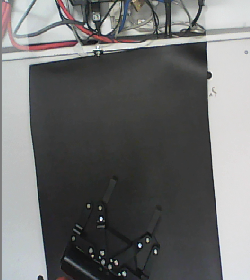
\includegraphics[width=0.3\linewidth]{backgrond} %
		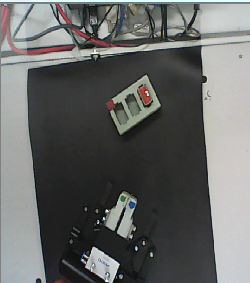
\includegraphics[width=0.3\linewidth]{base} %	
			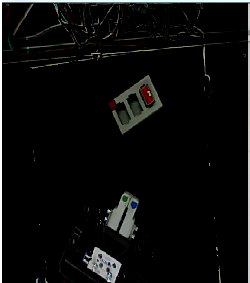
\includegraphics[width=0.3\linewidth]{diff}
	\caption{ Background image, new capture with objects in place and resulting subtraction }
	\label{fig:backgrond}
\end{figure}\ \\
This image was then converted to a binary matrix, with a threshold of each colour layer, and a a grey scale process, to combine the colour layers. This process is shown in \cref{fig:out2}.\\ 
\begin{figure}\centering
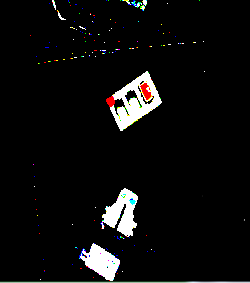
\includegraphics[width=0.3\linewidth]{out1} %
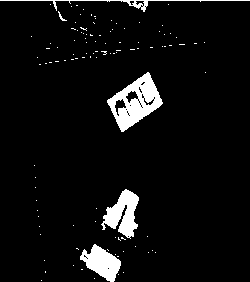
\includegraphics[width=0.3\linewidth]{out2}
\caption{Threshold of each colour, and combining of colour layers to make single layer binary}
\label{fig:out2}
\end{figure}
\begin{figure}
	\centering
	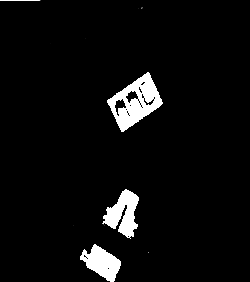
\includegraphics[width=0.3\linewidth]{out4}
	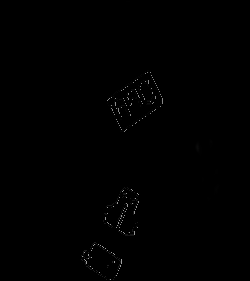
\includegraphics[width=0.3\linewidth]{out3}
	\caption{Erode and Dilate removes static from image, and Canny edge detection leaves only the outline of the objects }
	\label{fig:out4}
\end{figure}

The resulting image was then eroded and dilated by one pixel layer. This erode function turns any white pixel touching to a black pixel into a black pixel, while the dilate function performs the opposite. This resulted in any small imperfections being removed from the image, while only slightly reducing the object recognition quality of the image. This is seen in \cref{fig:out4}(a).

A Canny edge detection was then used, which finds object edges by leaving only white pixels that are touching black pixels behind. The resulting image is shown \cref{fig:out4}(b).

Each group of remaining white pixels was now classified as a contour, via the \textit{findContours} command. This process found any collection of white pixels as a polygon shape. It also listed the contour hierarchy, where contours are set as parents, and any contours inside its pixel range are defined as its children. The main holding box, and the gripper, are both objects not encased in larger objects. Therefore, only contours with no parents were further examined.\\

Each contour examined was fitted inside a rectangle with \textit{minAreaRect}. This found the smallest rectangle, of any angular orientation, that could fit the whole contour. The size of this rectangle was then tested, anything outside the set threshold was ignored.\\
For each rectangle that was within the predicted size of the holding box or gripper, a classification and orientation was attempted as if the object were a holding box. If this process failed, the image was oriented as a gripper. If this failed, the object was deemed neither and discarded. From the example process, at the stage in \cref{fig:out4}(b), three objects remain; the holding box, the gripper and another part of the gripper of no interest.  Respectively, these objects would be assigned as a holding box; fail at being set as a holding box, and be assigned as a gripper, and fail at both assignings.\\
This process is shown in diagram in \cref{fig:Throwlinek}.
\begin{figure}[h]
\centering
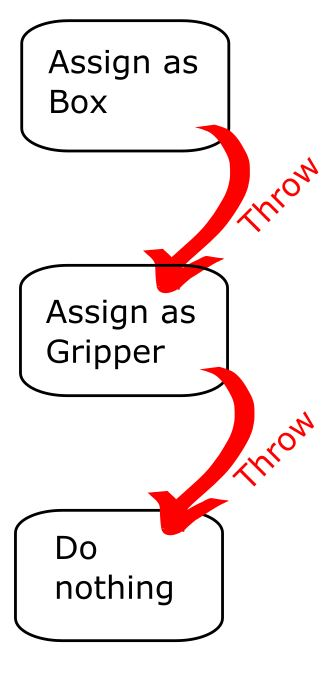
\includegraphics[width=0.2\linewidth]{Throwlinek}
\caption{Assigning process through try, catch, throw}
\label{fig:Throwlinek}
\end{figure}

\subsection{Object orientation}

Both the holding box and gripper are recognised in this process as \mbox{\textit{RotatedRect}s} these are open-cv objects which consist of a size, angle and centre coordinate. However, the four corner points can be extracted from the object. When orientating as a holding box, each of these corners has the surrounding pixels examined, with the corner that has the highest ratio of red being deemed the reference corner. This reference corner is shown in figure \cref{fig:Redest}. To derive the highest red ratio \cref{eq:redest} was used. By referencing the corner with the most red \textit{ratio} rather than highest red mean, a white corner is not incorrectly identified. If a corner of a set red ratio value is not found, the classification as a holding box is aborted, and a gripper is tried, as discussed above.
\begin{equation}
mean(red)/(mean(blue)+mean(green)+mean(red))
\label{eq:redest}
\end{equation}
\begin{figure}[h]
	\centering
	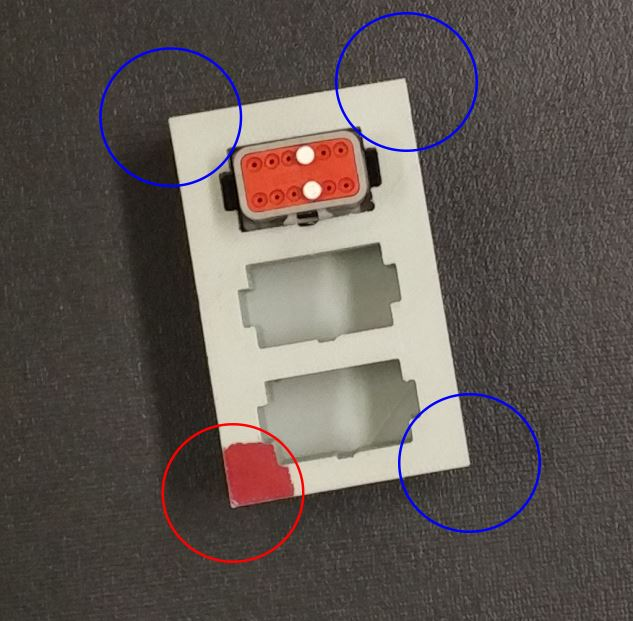
\includegraphics[width=0.3\linewidth]{Redest}
	\caption{Red detection for reference corner}
	\label{fig:Redest}\end{figure}\\

This reference corner was then used to determine the holding box true angle in relation to the camera. This is required as the angle of the RotatedRect is only in the range 0$^{\circ}$ to -90$^{\circ}$. Shown in  \cref{fig:angleissue}, the RotatedRect is initially a short, wide rectangle at -20$^{\circ}$. However, when rotated by -80$^{\circ}$ the RotatedRect becomes a tall, thin rectangle at -10$^{\circ}$. To rectify this, the index of the reference corner from the list of corners returned from the RotatedRect function was examined, and the true angle was found with an addition of 0, 90$^{\circ}$, 180$^{\circ}$ or 270$^{\circ}$. 

\begin{figure}[h]
\centering
\includegraphics[width=0.7\linewidth]{"angle_issue"}
\caption{}
\label{fig:angleissue}
\end{figure}

This orientation process is repeated for the gripper arm, but using the blue and green dots on the gripper fingers. 
	
\section{Pin detection and PinHole Allocation}
With the holding box true angle determine, a copy of the image could be rotated and cropped to be only the holding box. This cropping can be seen in \cref{fig:holdingblockwithdata}.
\begin{figure}[h]
	\centering
	\includegraphics[width=0.3\linewidth]{"holding_block_with_data"}
	\caption{Holding box image, cropped down to only the box, and with all socket overlay shown}
	\label{fig:holdingblockwithdata}
\end{figure}\\
Data on this holding box could now be used to find the sockets in the holding box.\footnote{At this point, hard coding has been used, however if several holding boxes are used in future development, a bar code system will be introduced for identification and CSV extraction use.} This information defines how large the box is in millimetres, so a pixel per millimetre ratio can be found. The box information also defines where the sockets should be (in millimetres), within the box.\\
By using the ratio, and the physical displacement of each socket, a \textit{socket} object was made. Each socket object was passed the holding box image, its pixel starting point within this image, expected hight, and file name for CSV file with pin details. The socket started by cropping a reference matrix of the box image to only the useful area. Using reference copies, or \textit{shallow copies}, has two main advantages: Firstly, the memory used  and copy execution time is reduced, as the socket's stored \textit{Mat} is only a pointer, not a whole new matrix. Secondly, the socket image can be edited for user feedback, and the original holding box image is effected. This allows only a holding box to be presented to the user with all socket information being shown, rather than loading each socket image separately. An example of this is shown in \cref{fig:holdingblockwithdata}. \\
Using its sub-matrix, the socket examined the mean red ratios, as used for the holding box corner, and determines if a socket was present, as shown in \cref{fig:fullSock}.
\begin{figure}[h]
\centering
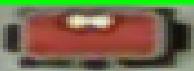
\includegraphics[width=0.4\linewidth]{fullSock} %
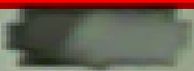
\includegraphics[width=0.4\linewidth]{emptySock}
\caption{Active and empty socket place identified and presented with, respectively, green or red bar above}
\label{fig:fullSock}
\end{figure}\\

Sockets that have been identified as present are then further examined to find the exact area for pin hole mounting. Shown in \cref{fig:sock1} is the original socket image. A threshold function of high red, low green, low blue is performed, \cref{fig:sock2}. The image is eroded and dilated, \cref{fig:sock3}, and a canny edge detection is conducted, \cref{fig:sock4}. The image is then cropped to fit the resulting contour, \cref{fig:sock5}.\\

\begin{figure}[h]
	\centering
	\begin{subfigure}{0.3\linewidth}
		\centering
		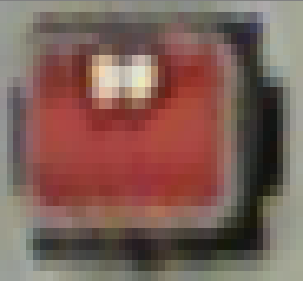
\includegraphics[width=\linewidth]{sock1}
		\subcaption{original sub-matrix}
		\label{fig:sock1}
	\end{subfigure} \hspace{0.2\linewidth}
	\begin{subfigure}{0.3\linewidth}
		\centering
		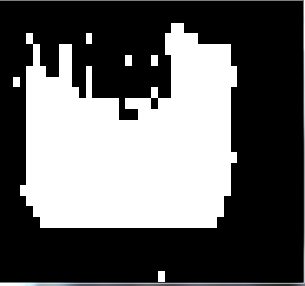
\includegraphics[width=\linewidth]{sock2}
		\subcaption{Post-threshold}
		\label{fig:sock2}
	\end{subfigure}
	\begin{subfigure}{0.3\linewidth}
		\centering
		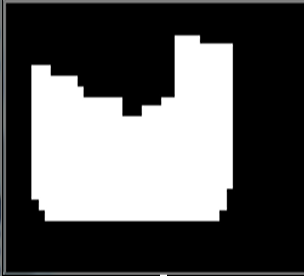
\includegraphics[width=\linewidth]{sock3}
		\subcaption{Small specs removed}
		\label{fig:sock3}
	\end{subfigure}\hspace{0.2\linewidth}
	\begin{subfigure}{0.3\linewidth}
		\centering
		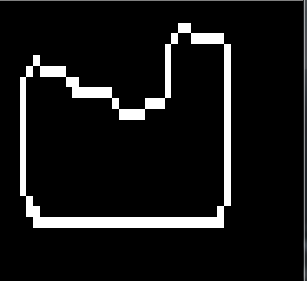
\includegraphics[width=\linewidth]{sock4}
		\subcaption{Edge detection}
		\label{fig:sock4}
	\end{subfigure}
	\begin{subfigure}{0.3\linewidth}
		\centering
		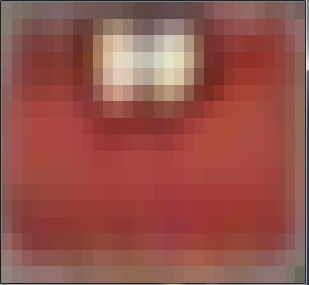
\includegraphics[width=\linewidth]{sock5}
		\subcaption{Matrix refit to edge of red area}
		\label{fig:sock5}
	\end{subfigure}\hspace{0.2\linewidth}
	\begin{subfigure}{0.3\linewidth}
		\centering
		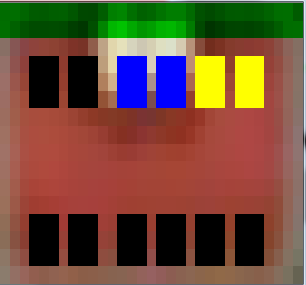
\includegraphics[width=\linewidth]{sock6}
		\subcaption{Pins identifed}
		\label{fig:sock6}
	\end{subfigure}
	\caption{Image processing of socket}
\end{figure}

Using a CSV dataset, the locations of the pins is then assigned. \note{may be able to add stuff here if better res camera allows us to have an extra layer of positioning}
The newly allocated pin hole is examined to find if a pin is present. To do this, the mean value of all three colour channels is compared with the 3 mean channels of the socket, if it is 25\% greater, a (white) pin is determined to be present.\\
A second CSV file then provides information on which pin holes should be filled. The resulting pin layout is shown in \cref{fig:sock6}, black pin holes are not filled, and should not be, blue have already been filled, and yellow still need to be filled.
 \FloatBarrier

\section{Path creation}
\subsection{Gripper to pin path creation}
With the pin holes assigned, the next available pinhole is requested from the main function. To do this, each layer between the main image and the pin holes are re-framed within their parent.\\
To begin, the first unfilled pinhole (coloured yellow above) reports to its parent socket the location within the socket. The socket then combines this location, and the location of the socket within the parent holding box, and reports this value to its parent holding box. \\
The holding box then re-orientates this coordinate to the global frame, and combines it with the holding box's location in the global frame. This final, global position of the pin is then reported to the main function.
A diagram of this process is shown in figure \cref{fig:aaah}.
\begin{figure}[h]
\centering
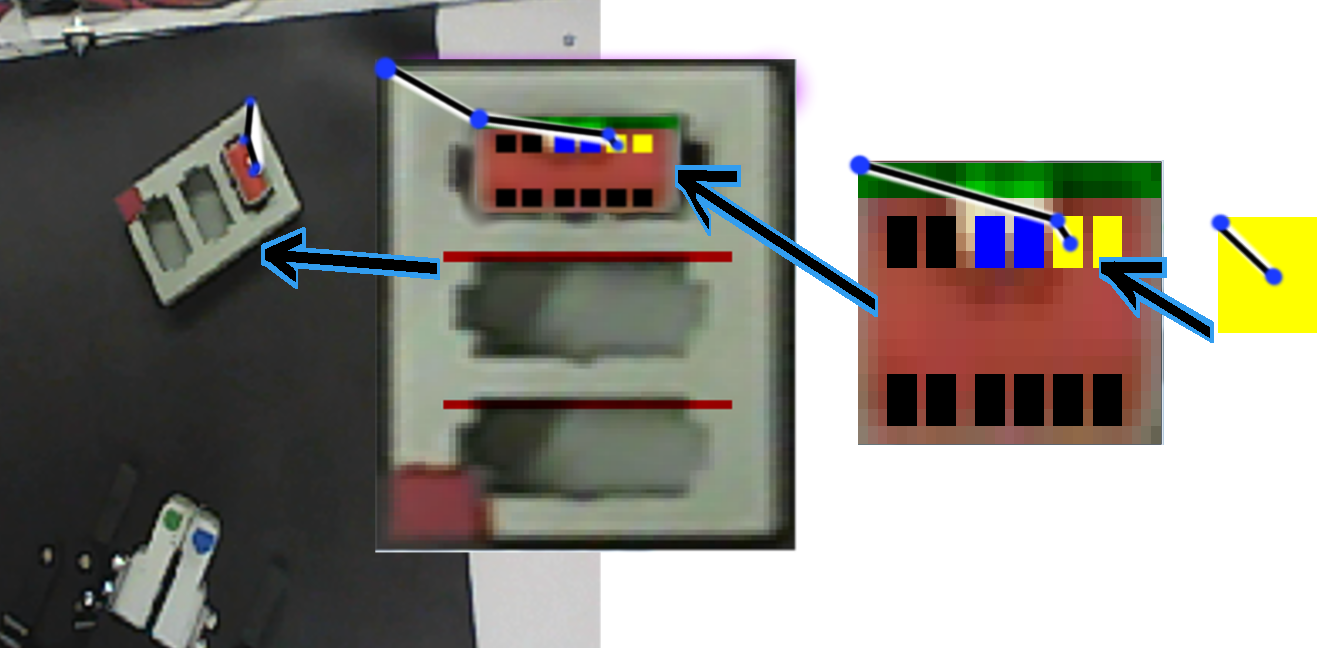
\includegraphics[width=\linewidth]{aaah}
\caption{Local position, cascading to parent to find global pin position}
\label{fig:aaah}
\end{figure}

The gripper single point coordinate is then determined by taking the half-way point between the green and blue corners of the gripper.\\

With the two singularity points for the gripper and pin identified, a vector is derived between them. This vector is given a magnitude and angle, and displayed to the user, as shown in \cref{fig:vector}.
\begin{figure}[h]
\centering
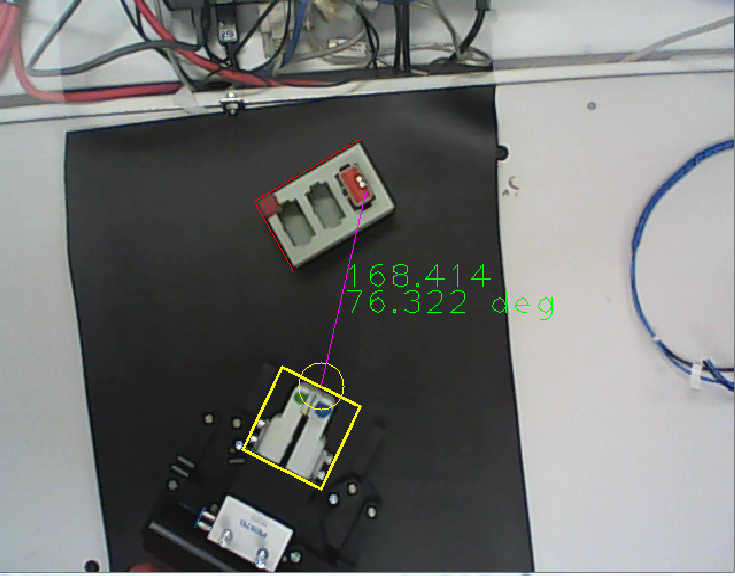
\includegraphics[width=0.5\linewidth]{vector}
\caption{Gripper to pin hole vector display}
\label{fig:vector}
\end{figure}
 \FloatBarrier

\subsection{Measurement correction}
As this application is being deployed under fluorescent lighting, there is some oscillation in lighting of the holing box and gripper. From this, the measurements recorded above cannot be assumed to be completely accurate. The graph shown in \cref{fig:measumrnetflux} shows that if the above \textit{object detection} and \textit{path measurement} process is repeated 30 times, in quick succession, there is a range of values recorded.\\ 

\begin{figure}[h]
\centering
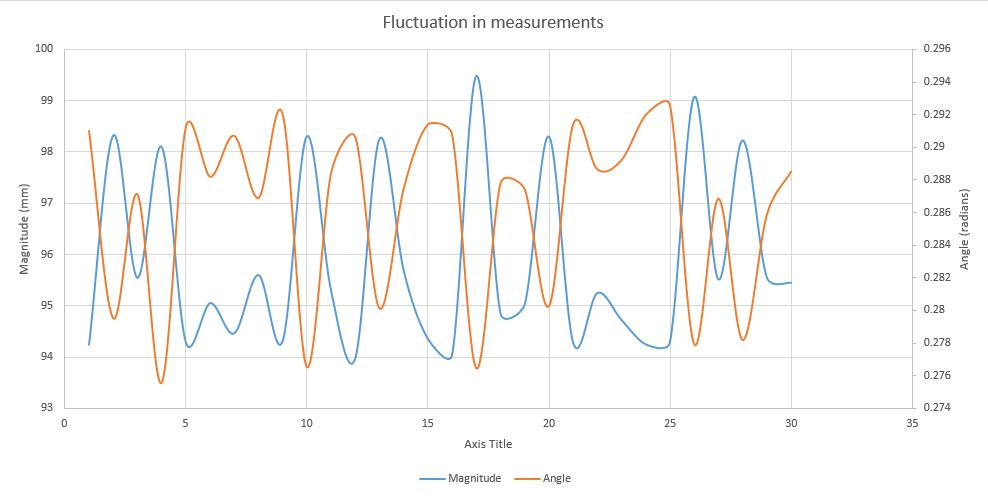
\includegraphics[width=0.7\linewidth]{measumrnetflux}
\caption{Vector magnitude and angle change over 30 records in close precession}
\label{fig:measumrnetflux}
\end{figure}
To reduce this lighting issue, the maximum and minimum values observed in this graph are taken, and averaged to derive an error reduced measurement. 
 
\subsection{Path to gripper arm co-ordinates}
\note{Vector converted to gripper co-ordinates.} 

To move the gripper towards its target pin-hole destination for placement, the robot-space position of the pin hole must be known. To find this, the camera-space pixel position of the pin hole is broken down into perpendicular component vectors (aligned to world axis) and then transformed into robot-space.

The following assumptions about the camera and workspace were made to simplify the design of the pixel to robot-space conversion.
\begin{itemize}
	\item No camera distortion is present
	\item The effects of field-of-view and perspective can ignored due to the heads-down and mainly depth-agnostic nature of the workspace
	\item The z-position of target pin-hole is constant and known
\end{itemize}

A vector Xc aligned to x-axis of the robot-space is found in terms of camera-space. This is done by taking a photo of the robot gripper and noting the vector between its image position at x,y,z = (0,0,0) and at x,y,z = (200mm,0,0) during the calibration phase of the program. This allows for decomposition of the gripper-to-pin-hole vector Pc into terms of perpendicular vectors Xc and Yc (y axis). To find these Pc components the following equations are used. 

\begin{equation}
Pcx*Xc = (Xc.Pc)/(|Xc||Xc|)Xc
\label{eq:redest}
\end{equation}

\begin{equation}
Pcy*Yc = Pc - Pcx*Xc
\label{eq:redest}
\end{equation}

These vectors are the pixel space components aligned to world-space axis. To obtain the world-space scaled vector of the pin-hole Pw, the constants Pcx and Pcy are multiplied by the pixel to world scaling factor (200mm / the magnitude of Xc (pixels)). The gripper can now be commanded to move the transformed world pin-hole position Pw for placement of pin.


\chapter{Robotic Arm Control}

\section{Open ABB}
For this project, a basic parallel port was available for communication between the computer vision and the robotic arm. The parallel port allowed for single bits to be used as flags which triggered the robotic arm to perform action sets. For this project we needed to send specific travel distinations from the computer vision, to the robtic arm, therfore a more advance communication was required. To achieve this, OpenABB \footnote{$https://github.com/robotics/open_abb$} was used. This system has the robotic controller running a basic TCP server via RAPID code. A python script is used on the computer to connect to this server, and send commands. One such command can move the gripper to any point in the arms \hl{range/ field of operations, something like that} by sending the three axis coordinates.\\
This command list was extended by the team to  include gripper control and moving about the x and y axis, relative to the current position. 
An example of the command stack is shown in \cref{fig:commstack1}.
\begin{figure}[h]
\centering
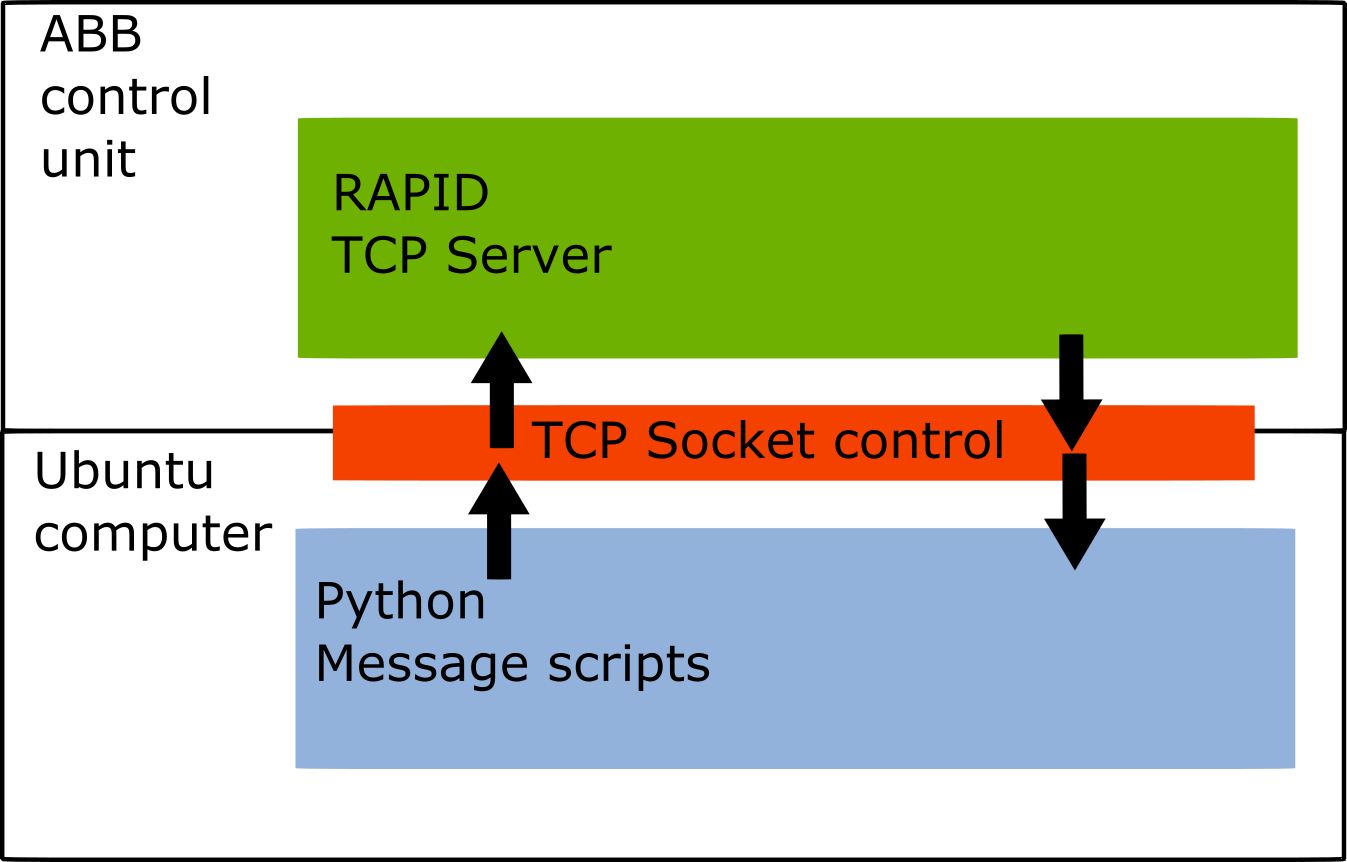
\includegraphics[width=0.7\linewidth]{commstack1}
\caption{Communication layers of OpenABB}
\label{fig:commstack1}
\end{figure}

\section{Coordination}
As the computer vision was made in c++, and the openABB c++ code requires a full ROS installation, it was instead chosen to implement a python calling system in c++. This interface called a python run-time, and sent commands via $PyRun_SimpleString$.\\
The command stack was thus extended as shown in \cref{fig:commstack2}
\begin{figure}[h]
\centering
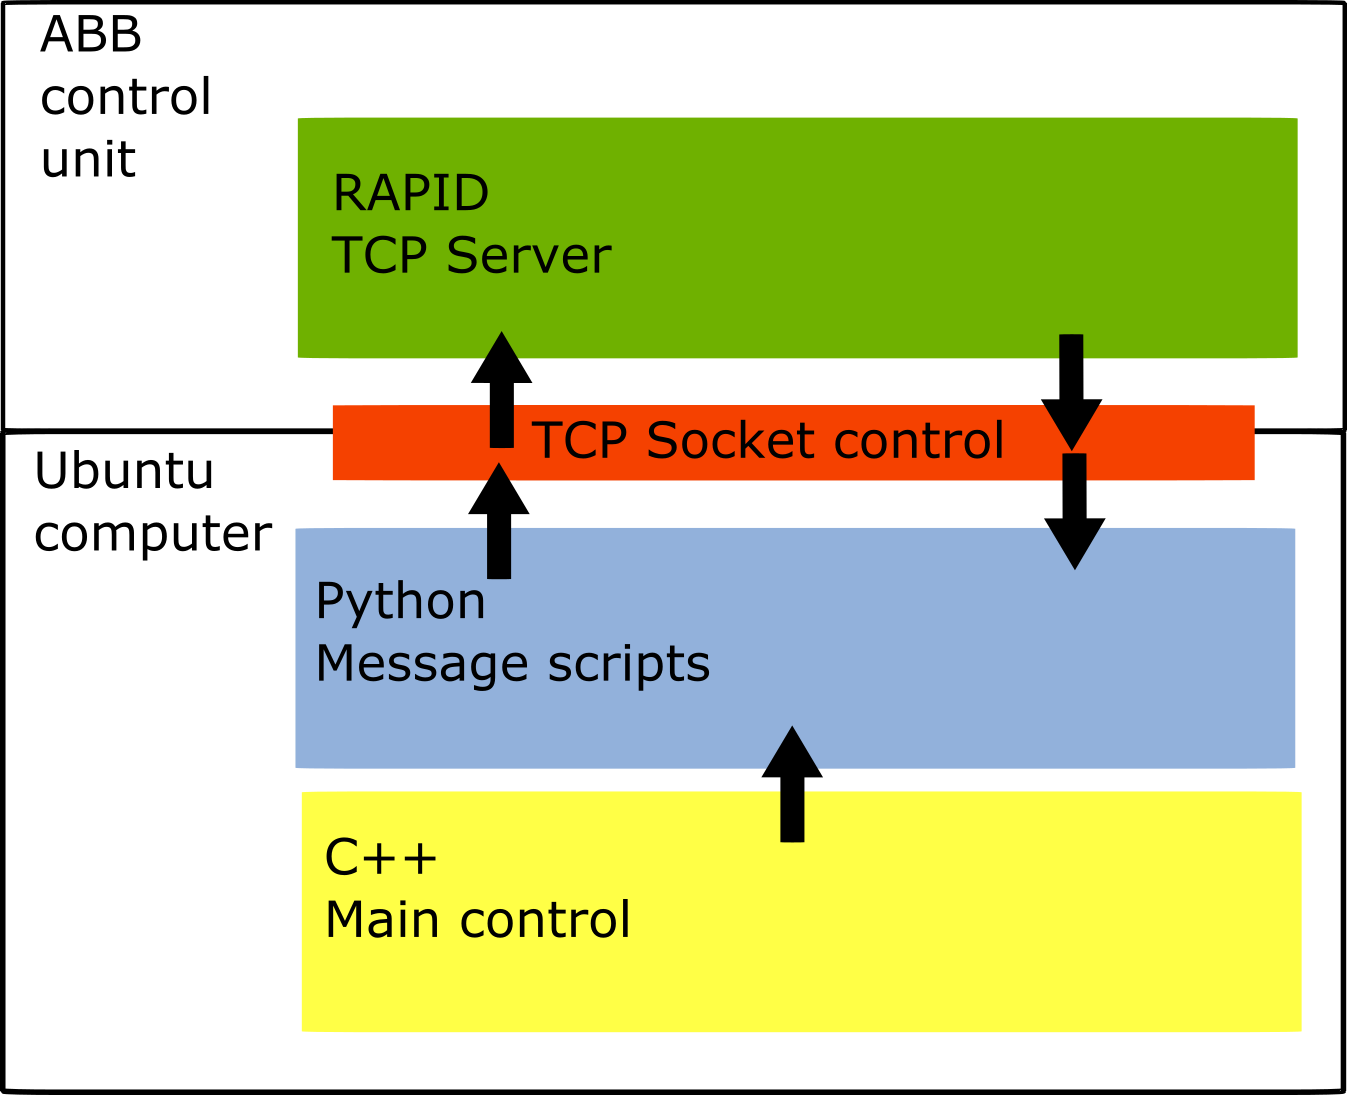
\includegraphics[width=0.7\linewidth]{commstack2}
\caption{Communication stack with added c++}
\label{fig:commstack2}
\end{figure}
 
\chapter{Operation Flow}
With the system's ability to know where to move to, and the ability to coordinate these movements, the operation flow charts can now be presented. Figure \ref{mainFlow} shows the standard operation flow, with purple action points being computer vision processes, and pink being robotic arm actions. Figure \ref{calFlow} shows the operation for calibrating the difference between robotic arm frame, and the camera frame. 
%\pagenumbering{gobble}
\tikzstyle{decision} = [diamond, draw, fill=white!20, 
text width=4.5em, text badly centered, node distance=3cm, inner sep=0pt]

\tikzstyle{block} = [rectangle, draw, fill=red!20, text width=5em, text centered, rounded corners, minimum height=4em]
\tikzstyle{line} = [draw, -latex']
\tikzstyle{cloud} = [draw, rectangle,fill=blue!20,  text width=5em, text centered, rounded corners, minimum height=4em]
\tikzstyle{end} = [draw, rectangle,fill=white!20,  text width=5em, text centered, rounded corners, minimum height=4em]
\begin{figure}
\vspace*{-4cm}
\hspace*{-3cm}
\begin{tikzpicture}[node distance=2cm]
\node [end] (begin){Start};
\node [block, below of =begin] (start) {Move to postions 'Zero'};
%\node [block, right of= start, node distance=3cm] (calabrate) {Calabration of camera to gripper frame};
\node [cloud, below of = start] (image11) {Update image};
\node [cloud, right of=image11, node distance=3cm] (image12) {Object detection};
\node [decision, below of=image11, node distance=2.5cm] (decide3) {Is there a pin to place?};
\node [cloud, below of=decide3, node distance=3.5cm] (image13) {Measure pin distance};
\node [decision, below of=image13, node distance=3cm] (decide) {Enough measurements made?};
\node [cloud, below of=decide, node distance=3.5cm] (image21) {Average measrument};
\node [cloud, right of=image21, node distance=3cm] (image22) {Dump measurements};
\node [cloud, right of=image22, node distance=3cm] (image23) {Convert to robotic arm coordinates};
\node [block, below of=image21, node distance=2.5cm] (pinget1) {Move to pin supply};
\node [block, right of=pinget1, node distance=3cm] (pinget2) {Close gripper};
\node [block, below of=pinget1, node distance=2.5cm] (pinset1) {Move to pin hole};
\node [block, right of=pinset1, node distance=3cm] (pinset2) {Lower gripper};
\node [block, right of=pinset2, node distance=3cm] (pinset3) {Open gripper};
\node [block, right of=pinset3, node distance=3cm] (pinset4) {Raise gripper};
\node [block, right of=pinset4, node distance=3cm] (pinset5) {Move flat section over pin-head};
\node [block, right of=pinset5, node distance=3cm] (pinset6) {Lower gripper (4mm less)};
\node [end, right of=decide3, node distance=5cm] (Finish) {Finish} ;

\path [line] (begin) -- (start);
\path [line] (start) -- (image11);
\path [line] (image11) -- (image12);
\path [line] (image12) |- (decide3.north);

\path [line] (decide3) -- node [left]{yes} (image13);
\path [line] (decide3) -- node [above] {no} (Finish);

\path [line] (image13) -- (decide);
\path [line] (decide.west) -| ++(-0.5,6) node [right] {no} |- (image11.west);
\path [line] (decide) -- node [left] {yes} (image21);
\path [line] (image21) -- (image22);
\path [line] (image22) -- (image23);
\path [line] (image23.south) -- ++(0,-0.5) -|  (pinget1);

\path [line] (pinget1) --  (pinget2);
\path [line] (pinget2) |- ++(-1,-1.25) -| (pinset1.north);
\path [line] (pinset1) --  (pinset2);
\path [line] (pinset2) --  (pinset3);
\path [line] (pinset3) --  (pinset4);
\path [line] (pinset4) --  (pinset5);
\path [line] (pinset5) --  (pinset6);
\path [line] (pinset6.south) |- ++(-18,-0.5) |- (start);
\end{tikzpicture}

\caption{Main Process} \label{mainFlow}
\end{figure}

\begin{figure}
	\begin{tikzpicture}
	\node [end] (begin){Start};
\node [block, below of =begin, node distance=2cm] (start) {Move to postions 'Zero'};
	\node [cloud, right of= start, node distance=3cm] (calabrate1) {Update image};
	\node [cloud, right of= calabrate1, node distance=3cm] (calabrate2) {Object detection};
	\node [cloud, right of= calabrate2, node distance=3cm] (calabrate22) {Measure gripper location in camera};
	\node [decision, right of=calabrate22, node distance=4cm] (decide) {Enough measurements made?};
	\node [cloud, below of=start, node distance=3cm] (image1) {Average measrument};
	\node [cloud, right of=image1, node distance=3cm] (image12) {Dump measrument};
		
	\node [block, below of= image1, node distance=3cm] (calabrate3) {Move 200 along X-axis};
	\node [cloud, right of= calabrate3, node distance=3cm] (calabrate4) {Update image};
	\node [cloud, right of= calabrate4, node distance=3cm] (calabrate5) {Object detection};
		\node [cloud, right of= calabrate5, node distance=3cm] (calabrate52) {Measure gripper location in camera};
	\node [decision, right of=calabrate52, node distance=4cm] (decide2) {Enough measurements made?};
	\node [cloud, below of=calabrate3, node distance=3cm] (image2) {Average measrument};
	\node [cloud, right of=image2, node distance=3cm] (image22) {Dump measrument};
	\node [end, below of=image2, node distance=2.5cm] (Finish) {Finish} ;
	
	\path [line] (begin) -- (start);
	\path [line] (begin) -- (start);
	\path [line] (start) -- (calabrate1);
	\path [line] (calabrate1) -- (calabrate2);
		\path [line] (calabrate2) -- (calabrate22);
	\path [line] (calabrate22) -- (decide);
	\path [line] (decide.south) node[below]{yes} -| (image1.north);
	\path [line] (decide.north) node[above]{no}  -|  (calabrate1.north);
	\path [line] (image1) -- (image12);
	\path [line] (image12.south) -- ++(0,-0.2)-| (calabrate3.north);
	\path [line] (calabrate3) -- (calabrate4);
	\path [line] (calabrate4) -- (calabrate5);
		\path [line] (calabrate5) -- (calabrate52);
		\path [line] (calabrate52) -- (decide2);

			\path [line] (decide2.south) node[below]{yes} -| (image2.north);
			\path [line] (decide2.north) node[above]{no}  -|  (calabrate4.north);
		\path [line] (image2) -- (image22);
		\path [line] (image22.south) -- ++(0,-0.2)-| (Finish.north);
	\end{tikzpicture}
\caption{Calibration} \label{calFlow}
\end{figure}
\chapter{Matlab Simulation}
\section{Denavit-Hartenberg Algorithm}
\begin{table}[h]

	\centering
	\begin{tabular}{| l | c c c c c |}
		\hline
		Links 	& $\theta$ 		& d 	& a 	& $\alpha$	& Physical	\\ [0.5ex]
		\hline
		1 		& $\theta$ 		& 0 	& 0 	& 0 		& Base 		\\
		2 		& $\theta$2 	& 0 	& 0.07 	& $\pi$/2 	& Shoulder	\\
		3 		& $\theta$3 	& 0 	& 0.36 	& 0 		& Elbow		\\
		4 		& $\theta$4 	& 0.38 	& 0 	& $\pi$/2 	& Twist-1	\\
		5 		& $\theta$5 	& 0 	& 0 	& -$\pi$/2 	& Wrist		\\
		6 		& $\theta$6 	& 0.108 & 0 	& $\pi$/2 	& Twist-2	\\ [1ex]
		\hline
		
	\end{tabular}
		\caption{Denavit-Hartenberg Algorithm}
\end{table}

The Denavit-Hartenberg matrix above gives a close approximation to the movement and joint rotation behaviour of the ABB robot arm. Due to the nature of elbow and wrist rotations, a `d' offset is given for joints 4 and 6, allowing a rotation about the length of a previous link.\\
Assumptions are made with the position of joints 4 and 6, where joint 4 is located roughly in the middle of joints 3 and 5 on the physical robot, however since it's rotation is about the link axis it is irrelevant where this joint is located, so long as it is within the linkage length. That is to say, if this link is rotated by a joint at any point along its length, the rotational behaviour of further joints will be the same. Due to this behaviour, joint 4 can be simulated at one end of the robot's forearm, instead of at its physical location on the robot's forearm.\\
A problem occurs when attempting to set a joint which rotates about the link axis. When the Matlab link configuration has an `a' or `d' offset after any joint which rotates about a link axis, Matlab cannot construct the robot arm model correctly in the simulation. This is due to the `a' and `d' offset lengths both being perpendicular to the link axis. In order to fix this problem and simplify the Denavit-Hartenberg algorithm, it is easier to set the distance between joints 4 and 5 to zero then rotate joint 5 into the correct orientation.\\
It was also assumed that joint 6 can be located at the end-effector in order to benefit the simulation so that movements and translations will include that distance in calculations. This means that the link between joints 5 and 6 will simulate the end-effector.\\
Regardless of alterations made in order to simplify the algorithm notation or fix errors produced in a Matlab simulation, the motion characteristics are equivalent to the physical movements of the ABB robot.

\section{Matlab implementation}
The Matlab Robotic, Vision and Control library (RVC) is useful for mathematically representing configured links on a robot arm using Denavit-Hartenberg notation. When using the algorithm, links can be created by a user and added to a defined Robot object using the SerialLink() function.\\
A single position may be mapped using an array of elements equal to the amount of links. Each element represents either joint translation for prismatic joints or rotation for rotary joints. The order in which the joints are represented in the array need to be the same order in which the links were created in the Denavit-Hartenberg algorithm. For the ABB robot, only rotational joints are present.\\
To begin with, a starting position is defined for robot arm joint rotation, in this case all angles are set to zero degrees, which represents the unmodified model of the Denavit-Hartenberg algorithm. In this pose it is easy to see whether or not the joints are configured correctly and that the model does in fact mirror the basic shape of the physical model being simulated.\\
The next step is to define the x,y,z position and rotation for each point of motion which will be simulated. This can be done by simply assigning variables to represent that information as in \cref{Matlab}, lines 45-105. In order to run an effective simulation, the position and rotations must be compiled into a transformation matrix. This matrix defines all translational and rotational movement required between the reference frame and the desired destination frame. In order to convert the raw variables representing the position and rotation of the end-effector into a transform matrix, two functions are used. One is transl(x,y,z), which represents translation and takes in the x, y and z position of a point and the other is rpy2tr(rx,ry,rz), which represents the roll, pitch and yaw angle which rotate about x, y and z respectively. The result of these two functions are multiplied together and saved as the transformation matrix for the specified point, in the order as seen in \cref{Matlab}, lines 108-114. A transformation matrix for the initial position is also required. This is achieved easily by using the forward-kinematic function fkine(q), where q is a 1xn array representing the joint rotations where n is the number of joints on the robot arm.\\
In \cref{Matlab}, lines 121-126, two arrays are initiated. The first one is a mask representing the degrees of freedom available in the joint path calculations. The second array represents a joint angle position array which acts as a reference point. This point is useful by forcing the movement of the arm to conform to the specified joint angles. This helps to simulate movement that stays within the bounds of the work area of the robot. As a solution for each joint converges with the corresponding reference angle, the angles will only change when a joint has the least convergence.\\
Although we have a transformation matrix for each position we wish to simulate, what we really need are the joint angles values in radians, which are the exact rotations of every joint which together correspond to the position of the end-effector. In order to get a joint angle array from a transformation matrix, we can use the inverse-kinematic function ikine(T,qr,M), where T is a transformation matrix for the point, qr is the reference array used to restrict motion and M is the mask for the degrees of freedom available. For the ABB robot, the joint angles at the simulated points are calculated as in \cref{Matlab}, lines 121-135. When finding the inverse kinematic of the transformation matrix, the function ikine() takes into account the reference array and the degrees of freedom in order to find a single solution for the joint angle configuration which makes up the desired position and rotation. Users must be careful, however, as having an inappropriate reference array may cause the calculations to diverge, resulting in sub-optimal solutions which may even result in simulation movement outside of the immediate work area.\\ 
 

\appendix
\chapter{Matlab Code}
\label{Matlab}
\definecolor{mygreen}{RGB}{28,172,0} % color values Red, Green, Blue
\definecolor{mylilas}{RGB}{170,55,241}
\lstset{language=Matlab,%
    %basicstyle=\color{red},
    breaklines=true,%
    morekeywords={matlab2tikz},
    keywordstyle=\color{blue},%
    morekeywords=[2]{1}, keywordstyle=[2]{\color{black}},
    identifierstyle=\color{black},%
    stringstyle=\color{mylilas},
    commentstyle=\color{mygreen},%
    showstringspaces=false,%without this there will be a symbol in the places where there is a space
    numbers=left,%
    numberstyle={\tiny \color{black}},% size of the numbers
    numbersep=9pt, % this defines how far the numbers are from the text
    emph=[1]{for,end,break},emphstyle=[1]\color{red}, %some words to emphasise
    %emph=[2]{word1,word2}, emphstyle=[2]{style},
     xleftmargin=-0.1\linewidth,
    linewidth=1.2\linewidth,       
}

\begin{lstlisting}
% Simple example of using the Matlab Robot toolbox v9.9 for RME40003 Robot 
% Systems Design, 2014.
%
% The example is for a three-link RPR manipulator that was covered in the 
% lectures and the tutorials.
%
% Example developed by M. Dunn, 2014, Swinburne University of Technology,
% Melbourne, Australia
%
% References::
% - Robotics, Vision & Control, Chap 7
%   P. Corke, Springer 2011.

clear L

%% Define the link parameters for the manipulator
% Set the fifth parameter as 0 for a rotary joint, 1 for a prismatic joint
% Set the "modified" flag to true (we are using the modified
% Denavit-Hartenberg convention in RME40003)

sF = 1.0;
%             theta   d      a       alpha   R(0)/P(1)
L(1) = Link([ 0       0      0       0       0], 'modified');
L(2) = Link([ 0       0      0.07    -pi/2   0], 'modified');
L(3) = Link([ 0       0      0.36    0       0], 'modified');
L(4) = Link([ 0       0.38   0       -pi/2   0], 'modified');
L(5) = Link([ 0       0      0       pi/2    0], 'modified');
L(6) = Link([ 0       0.108  0       -pi/2   0], 'modified');

%% Set up the manipulator
robot = SerialLink(L, 'name', 'RME40003 Project');

%% Define some poses
%start pose
q0 = [     0, -pi/4, -pi/4,     0,     0,     0]; 

% 1:Base-rot
% 2:shoulder-rot
% 3:elbow-rot
% 4:elbow-twist
% 5:wrist-pivot
% 6:wrist-twist


%% Raw position and rotation data for each point
%point1

x1 = 0.273/sF;
y1 = -0.740/sF;
z1 = 0.02/sF;

%radians
rotx1 = pi;
roty1 = 0;
rotz1 = 0;

%point2
x2 = 0.273/sF; 
y2 = -0.740/sF;
z2 = -0.1/sF;

%radians
rotx2 = pi;
roty2 = 0;
rotz2 = 0;

%point3
x3 = 0.273/sF;
y3 = -0.740/sF;
z3 = 0.02/sF;

%radians
rotx3 = pi;
roty3 = 0;
rotz3 = 0;

%point4
x4 = 0.4/sF;
y4 = -0.4/sF;
z4 = 0.02/sF;

%radians
rotx4 = pi;
roty4 = 0;
rotz4 = 0;

%point5
x5 = 0.4/sF;
y5 = -0.4/sF;
z5 = -0.1/sF;

%radians
rotx5 = pi;
roty5 = 0;
rotz5 = 0;

%point6
x6 = 0.4/sF;
y6 = -0.4/sF;
z6 = 0.02/sF;

%radians
rotx6 = pi;
roty6 = 0;
rotz6 = 0;


%% Point translation homogeneous matrixes
T1 = transl(x1,y1,z1)*rpy2tr(rotx1,roty1,rotz1);
T2 = transl(x2,y2,z2)*rpy2tr(rotx2,roty2,rotz2);
T3 = transl(x3,y3,z3)*rpy2tr(rotx3,roty3,rotz3);
T4 = transl(x4,y4,z4)*rpy2tr(rotx4,roty4,rotz4);
T5 = transl(x5,y5,z5)*rpy2tr(rotx5,roty5,rotz5);
T6 = transl(x6,y6,z6)*rpy2tr(rotx6,roty6,rotz6);


%% Find the forward kinematics of the pose
fk_q0 = robot.fkine(q0);


%% Find the inverse kinematics for fk_qs and fk_qe
% Set a mask for the degrees of freedom
M = [1, 1, 1, 1, 1, 1];

% Point set for forced convergence
qi = [0,-pi/4,-pi/4,0,pi/2,-pi/2];

% Calculate the inverse kinematics of each point
ik_q0 = robot.ikine(fk_q0,qi,M); %fk of initial angles, initial position estimation, DOF settings
ik_q1 = robot.ikine(T1,qi,M);
ik_q2 = robot.ikine(T2,qi,M);
ik_q3 = robot.ikine(T3,qi,M);
ik_q4 = robot.ikine(T4,qi,M);
ik_q5 = robot.ikine(T5,qi,M);
ik_q6 = robot.ikine(T6,qi,M);

%% Find the joint trajectory for ten steps between the two poses
% Set the number of points
num_points = 10;

% Moving from point to point
jt0_1 = jtraj(ik_q0,ik_q1,num_points);
jt1_2 = jtraj(ik_q1,ik_q2,num_points);
jt2_3 = jtraj(ik_q2,ik_q3,num_points);
jt3_4 = jtraj(ik_q3,ik_q4,num_points);
jt4_5 = jtraj(ik_q4,ik_q5,num_points);
jt5_6 = jtraj(ik_q5,ik_q6,num_points);
jt6_0 = jtraj(ik_q6,ik_q0,num_points);

% Set the workspace of the robot
robot.plotopt = {'workspace',[-1, 1, -1, 1, -1, 1]};

% Plot the animations
while 1
	robot.plot(jt0_1);
	pause(1);
	robot.plot(jt1_2);
	pause(1);
	robot.plot(jt2_3);
	pause(1);
	robot.plot(jt3_4);
	pause(1);
	robot.plot(jt4_5);
	pause(1);
	robot.plot(jt5_6);
	pause(1);
	robot.plot(jt6_0);
	pause(1);
end
\end{lstlisting}

\end{document}\grid
